\section{A Framework for Pre-Runtime RT Analysis}

\begin{frame}{Overview}
	\begin{itemize}
		\item We propose a framework to identify whether a NoC-based manycore can run a real-time application without deadline violations. 
		
		\item We implemented a couple of tools to automate our approach, which relies on the \textit{scheduling} of system resources --- computation and communication. 
		
		\item Scheduling tasks on a single-core CPU is not novel, as some existing solutions date back to the 80s~\cite{gusfield:1984}. 
		
		\item However, incorporating the I/O components of the system, managing interruptions, and addressing the needs of NoCs requires additional modeling.
	\end{itemize}
\end{frame}

\begin{frame}
	\begin{itemize}
	\item Our framework concerns dataflow applications, where tasks have data dependency on sensors, the network, data off-loading, or other tasks. 
	
	\item In addition, tasks must employ a variation of the predictable execution (PREM)~\cite{Senoussaoui:2022} and the logical execution time (LET)~\cite{Gemlau:2021} models; we divide tasks in \emph{receiving}, \emph{processing}, and \emph{sending} phases as the controlled execution of tasks is key for I/O access predictability. 
	
	\item We expect applications to have real-time requirements on (i) the iteration time and (ii) the number of iterations per second. The former is the end-to-end application execution time, which is particularly important in sensor applications as it dictates the accuracy of sensors in time, i.e., how old the reading is. The latter is the application execution rate, which relates to the periodic execution of tasks.
	\end{itemize}
\end{frame}

\begin{frame}
	\begin{figure}[!t]
		\centerline{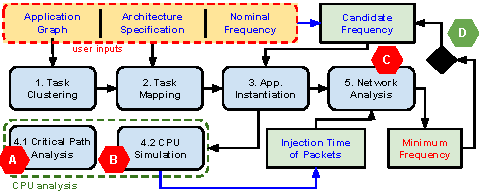
\includegraphics[width=0.8\columnwidth]{fig/workflow.pdf}}
		\caption{A workflow depicting our approach. User inputs appear at the top. Activities appear as blue shapes. Outcomes appear as green shapes. Tags A, B, and C represent activities of the workflow that may fail due to the unavailability of system resources. Tag D represents the end of the workflow, where users can choose to abandon the workflow or further optimize the result.}
		\label{fig:workflow}
		\vspace{-12 pt}
	\end{figure}
\end{frame}

\begin{frame}

	The proposed framework (Figure~\ref{fig:workflow}) takes three inputs: (i) application graph, (ii) architecture specification, and (iii) nominal manycore frequency. 
	
	\begin{enumerate}
		\item[i)] We described applications using a directed, potentially cyclic, graph $G = (E, V)$, where $V$ is the set of vertices and $E$ is the set of edges. Vertices represent tasks, to which we tag the corresponding worst-case execution time (WCET), in cycles. Edges represent flows of data, i.e., a set of packets with periodic behavior, given by a $3$-tuple $f =\langle p, c, d \rangle$, corresponding to the period ($p$), capacity ($c$), and deadline of flows ($d)$, in clock cycles.
		\item[ii)] The architecture specification must describe a zero-load latency model of the network and a set of allowed operating frequencies for the manycore. Please note that the entire system runs at the same frequency.
		\item[iii)] The framework considers the nominal frequency as the start point for the frequency optimization. 
	\end{enumerate}
\end{frame}

\begin{frame}

	\begin{itemize}
		\item At the first iteration, the framework computes whether the nominal frequency suits the application. 
		
		\item The framework runs in interactive or automated modes. 
		
		\item In interactive mode, users must decide to increase the frequency (if the platform allows), try a lower frequency, or abandon the process at each iteration. 
		
		\item In automated mode, the framework runs until it reaches a given number of iterations or cannot optimize the frequency further, assuming a tolerance factor. 
		
		\item The framework evaluates the application at each iteration, using a 5-step analysis: (i) task clustering, (ii) task mapping, (iii) application instantiation, (iv) CPU analysis, and (v) network analysis. CPU analysis splits in critical path analysis (CPA) and CPU simulation.
	\end{itemize}

\end{frame}

% -------------------------------------------------------------------------------


\begin{frame}{1 - Task Set Clustering and Mapping}
	\begin{itemize}
	\item Task set clustering consists of splitting an application graph into multiple task sets to be assigned by the framework to a PE during the mapping step (Figure~\ref{fig:workflow}, step 1). 
	
	\item The goal is to generate one cluster per PE. We created an algorithm to cluster graphs that performs $O(n)$  on the number of vertices of the application task graph. 
	
	\item The algorithm iteratively removes edges from the graph, combining vertices until the resulting graph has $|$\textit{V}$| \leq |\text{\textit{PEs}}|$, based on one of two criteria. 
	
	\item The \textsc{min-comm} criterion reduces the overall network load, eliminating edges with the most communication load groups communication-intensive tasks in the same cluster. 
	
	\item Oppositely, the \textsc{max-proc} criterion balances the CPU usage between PEs by grouping tasks with the least CPU load. Once the algorithm computes the clusters, we can map them to the manycore using a task mapping strategy (Figure~\ref{fig:workflow}, step 2). 
	
	\item Note that task mapping is a well-developed topic in the literature~\cite{Singh:2013}, so discussing task mapping is out of the scope of this paper.
	\end{itemize}
\end{frame}

\begin{frame}{2 - Application Instantiation and Framework Loop}
	\begin{itemize}
		\item As the framework explores different frequencies during its execution, it must adjust the application parameters to match the frequency at each iteration (Figure~\ref{fig:workflow}, step 3). 
		
		\item The framework carries the WCET value of tasks along the multiple iterations, as the CPU architecture does not change. However, the framework must consider the periodicity of flows, adjusting the period and deadline of flows accordingly. 
		
		\item Iterations occur as follows. At the first iteration, the framework takes the nominal frequency as the candidate frequency, employing no adjustments to the application. 
		
		\item Based on the results of CPU analysis (Figure~\ref{fig:workflow}, step 4) and network analysis (Figure~\ref{fig:workflow}, step 5), the framework either increases or decreases the frequency. If the framework identifies violations of deadlines (tasks or flows), the candidate frequency will increase at the next iteration. 
		
		\item Similarly, the framework reduces the frequency if it detects no deadline violations. Searching for the minimum feasible frequency performs $O(log \ n)$, i.e., the time complexity of the binary search, where $n$ is the number of frequencies supported by the target platform (discrete).%GRAMMARLY-OK
	\end{itemize}
\end{frame}



\begin{frame}{3.a - Critical Path Analysis (CPA)}
	
	\begin{itemize}
		\item The CPU analysis is a 2-step process to assert that the manycore meets the CPU needs of an application. 
		
		\item The framework uses the CPA method~\cite{Kelley:1959} to evaluate the end-to-end processing time of an application iteration (Figure~\ref{fig:workflow}, step 4.1). 
		
		\item As PEs carry only subsets of the application task set, we must account for internal communication (task-to-task communication through memory spaces) and external communication (NoC). 
		
		\item The CPA method proceeds as Djkistra’s algorithm for computing the shortest path between two vertices~\cite{dijkstra:1959}, except that we multiply the weights of edges (communication load) by $-1$. 
		
		\item Although we cannot apply topological sort to cyclic graphs, we use depth-first search (DFS) to find and remove cycles, adding the weight of a removed edge to its origin vertex. 
		
		\item The result of this step is the number of cycles that the application takes to execute, i.e., the iteration time. The CPU must have enough cycles to run the application. Otherwise, the framework discards the candidate frequency and moves on to the next iteration.%GRAMMARLY-OK
	\end{itemize}
\end{frame}


\begin{frame}{3.b - Discrete-Event Simulation (DES) of PEs}
	
	\begin{itemize}
		
		\item The execution time of some kernel routines, e.g., dynamic memory allocation (\textit{malloc}) and interruption handling, is hard to predict. Our framework uses a DES engine to simulate PEs while assuming a worst-case characterization of kernel operations (Figure~\ref{fig:workflow}, step 4.2).
		
		\item It simulates PEs individually to find whether they can run the assigned task cluster. The simulation considers the WCET of the task scheduler, I/O interrupts, and other minor system-specific programmable interrupts. 
		
		\item If the framework detects that one of the PEs cannot run the assigned task set, the framework discards the candidate frequency and moves to the next iteration. 
		
		\item Due to the employment of the PREM and LET models, the framework can estimate the time in which tasks inject packets into the network. Packets enter the network only at the \textit{sending} phase, triggering an I/O event in the kernel. 
		
		\item The framework uses these values during the network analysis step (Figure~\ref{fig:workflow}, step 5) to predict the behavior of packets.
		
	\end{itemize}

\end{frame}



\begin{frame}{4 - Network Analysis}
	
	\begin{itemize}
		\item The network analysis occurs after the CPU analysis, considering that the framework kept the candidate frequency. 
		
		\item In this step, the framework asserts whether the network flows can traverse the NoC without deadline violations for a static set of flows. 
		
		\item Our flow model reassembles the Job-Shop model~\cite{Garey:1979}, where we replace machines with links (channels) and jobs with flits (data units). The goal of the network analysis step is to find a schedule for packets. The network analysis has 3 steps:
		
	\end{itemize}
\end{frame}

\begin{frame}{4 - Network Analysis (contd.)}
	
	
	\begin{enumerate}
		\item Unwrap flows to packets $p = \langle mrt, size, ad \rangle$, having a minimum release time ($mrt$), data size ($size$), and absolute deadline ($ad$) each. 
		
		\item Discover the path of packets in the NoC to compute the occupancy of links ($L$), i.e., a relation $O : P \times L \times T$, matching packets to the links they occupy in the discrete time domain (cycles), where $\forall p \in P$. 
		
		\item Find a schedule where the following constraints hold:
		\begin{itemize}
			\item[(\textsc{c1})] $prt \geq mrt$, where $ptr$ is the release time of packets in the found schedule;
			\item[(\textsc{c2})] $ad \geq prt + size / lw$, where $lw$ is the link width;
			\item[(\textsc{c3})] packets cannot overlap (single channel constraint);
			\item[(\textsc{c4})] flits of a same packet occupy the data bus one after another (wormhole constraint). 
			
		\end{itemize}
	\end{enumerate}
\end{frame}

\begin{frame}{Beware!}
	
	\begin{itemize}
		\item Generating a network schedule is NP-complete (similarly to job-shop).
		
		\item Instead, we use the $prt$ values collected during the CPU analysis, reducing the scheduling to a decision problem. 
		
		\item The framework indicates whether the schedule is feasible or not. If the schedule is feasible, the framework \textit{memorizes} the minimum frequency found so far. 
		
		\item Then, the framework can either try to find a lower frequency or abandon the process.%GRAMMARLY-OK
	\end{itemize}
	
\end{frame}